\documentclass[11pt]{article}
\usepackage[a4paper]{geometry}
\usepackage{polski}
\usepackage[utf8]{inputenc}
\usepackage{amsthm}
\usepackage[intlimits]{amsmath}
\usepackage{graphicx}
\usepackage{indentfirst}
\usepackage{float}
\usepackage[table,dvipsnames]{xcolor}
\usepackage[official]{eurosym}
\definecolor{LightCyan}{rgb}{0.88,1,1}

\title{Uczenie drzewa decyzyjnego na przykładzie wykrywania okularów na obrazach Olivetti}

\author{Karol Działowski}
\date{15.05.2019}
\begin{document}

\maketitle

\section{Opis problemu}

Celem zadania jest wykrywanie okularów na danych \emph{olivetti faces}. Klasyfikację przeprowadzono przy pomocy CART (classification and regression trees). Dane wejścowe zredukowano za pomocą analizy komponentów składowych (PCA).

W eksperymencie porównano wpływ na dokładność testową:
\begin{itemize}
\item liczby wymiarów danych (PCA)
\item użytych funkcji nieczystości
\item ograniczenia drzewa za pomocą głębokości
\item ograniczenia drzewa za pomocą procentu przykładów w liściu
\item ograniczenie drzewa za pomocą przycinania
\begin{itemize}
\item przy przeszukiwaniu wyczerpującym
\item przy przeszukiwaniu zachłannym
\end{itemize}
\end{itemize}

\begin{figure}[H]
\center
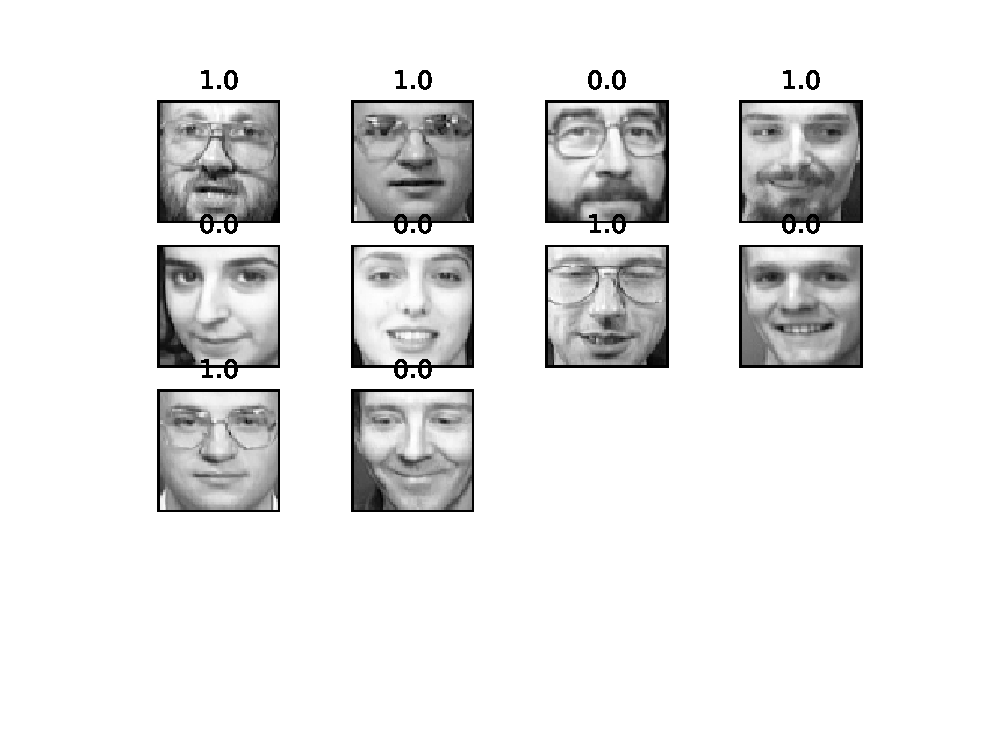
\includegraphics[width=0.6\textwidth]{predictions}
\caption{Przykład predykcji}
\end{figure}

\section{Wpływ na dokładność testową}

\subsection{Liczba cech danych}

Drzewo CART z funkcją nieczystości typu entropie uczono danymi o wymiarowościach $[15, 10, 15, 20, 25, 30, 35, 40, 45, 50, 55, 60, 65, 70]$ i porównano wpływ na błąd dla danych testowych.

\begin{figure}[H]
\center
\includegraphics[width=0.7\textwidth]{dimensions_test}
\caption{Liczba cech danych a dokładność testowa dla CART z funkcją nieczystości typu entropia }
\end{figure}

Dla 1małej ilości cech --- 10 wymiarów algorytm osiąga maksymalną dokładność, na poziomi 90\%. Przy zwiększaniu liczby cech do 25 dokładność maleje, by później znowu rosnąć do poziomi 87.5\% dla 30 i 40 cech.

\subsection{Wykorzystana funkcja nieczystości}

Porównano trzy funkcje nieczywości: entropia, indeks Giniego, błąd klasyfikacji.

Błąd klasyfikacji:
\begin{equation}
i(t) = 1 - \max_y P(y|t)
\end{equation}

Entropia:
\begin{equation}
i(t) = - \sum_y \frac{P(y|t) \cdot log_2 P(y|t)}{1}
\end{equation}

Indeks Giniego:
\begin{equation}
i(t) = 1 - \sum_y P^2(y|t)
\end{equation}

\begin{figure}[H]
\center
\includegraphics[width=0.7\textwidth]{dimensions_entropy_test}
\caption{Porównanie funkcji nieczystości}
\end{figure}

Najlepsze wyniki osiąga indeks Giniego, który dla osiąga minimalny błąd rzędu 10\%. Wyniki eksperymentu nie są przekonujące i nie można wysnąć oczywistych wniosków. 

\subsection{Ograniczenie głębokości}

Wykonany testy ograniczenia głębokości drzewa z funkcją nieczystości typu Entropia dla danych wejściowych o 50 cechach. Porównano wszystkie możliwe głębokości dla zbudowanego drzewa.

\begin{figure}[H]
\center
\includegraphics[width=0.7\textwidth]{depth_test}
\caption{Porównanie ograniczenia głębokości drzewa}
\end{figure}

Błąd testowy maleje wraz z wzrostem liczby poziomów drzewa i osiąga minimum dla głębokości równej 3. Dla głębokości 4 i 5, wyniki testów są minimalnie gorsze od minimum. Warto takie drzewo przyciąć na głębokość 3.

\subsection{Ograniczenie drzewa stosując procent przykładów}

Usunięto te węzły, które nie zawierały w sobie danego poziomu ogółu przykładów. Testowano drzewa z liściami które mają 10\% i mniej wszystkich przykładów. Porównanie przeprowadzono dla drzewa korzystającego z funkcji nieczystości typu entropia dla danych o 50 cechach.

\begin{figure}[H]
\center
\includegraphics[width=0.7\textwidth]{min_node_vals_test}
\caption{Porównanie ograniczenia minimalnego procentu przykładów w liściach}
\end{figure}

Osiągnięto minimum błędu testowego dla minimum 4\% i 3\% ogółu przykładów w węźle osiągając błąd 11.25\%. Osiągane wyniki są lepsze niż dla ograniczenia głębokości drzewa.

\subsection{Przycinanie drzewa}
\subsubsection{Przeszukiwanie wyczerpujące}

Porównano wpływ kar przy użyciu wyczerpującego przeglądania drzewa. Drzewo zbudowano dla danych o 50 cechach i przy użyciu funkcji nieczystości typu entropia.

\begin{figure}[H]
\center
\includegraphics[width=0.7\textwidth]{pruning_exhaustive}
\caption{Porównanie wpływu kar dla przycinania z przeglądaniem wyczerpującym}
\end{figure}


Zmiejszając karę za każdy liść błąd na danych uczących się zmniejsza, w pewnym momencie prowadząc do przeuczenia. Dla kary równej 0.10 błąd na danych testowych jest najmniejszy i wynosi 11.25\%, czyli osiągamy podobny wynik jak przy ograniczeniu stosując procent przykładów.

Średni czas budowania drzewa wynosił 6.1 sekundy.

\subsubsection{Przeszukiwanie zachłanne}

Porównano wpływ kar przy użyciu zachłannego przeglądania drzewa. Drzewo zbudowano dla danych o 50 cechach i przy użyciu funkcji nieczystości typu entropia.

\begin{figure}[H]
\center
\includegraphics[width=0.7\textwidth]{pruning_greedy}
\caption{Porównanie wpływu kar dla przycinania z przeglądaniem wyczerpującym}
\end{figure}

Zmiejszając karę za każdy liść błąd na danych uczących się zmniejsza, w pewnym momencie prowadząc do przeuczenia. Dla kary równej 0.10 błąd na danych testowych jest najmniejszy i wynosi 11.25\%, czyli osiągamy podobny wynik jak przy ograniczeniu stosując procent przykładów.

Średni czas budowania drzewa wynosił 4.5 sekundy. Zachłanne przeszukiwanie daje rezultaty zbliżone do przeszukiwania wyczerpującego (w naszym eksperymencie takie same) przy mniejszej złożoności obliczeniowej.

\section{Wnioski}

W eksperymencie porównano różne sposoby budowania drzewa CART na przykładzie danych \emph{olivetti faces}, których wymiarowość została zredukowana przy pomocy PCA. Przy odpowiednim stworzeniu drzewa można uzyskać dokładność na poziomie 90\% poprawnie przewidzianych klas na danych testowych.

\end{document}
